\documentclass[a4paper]{report}

% Some useful packages for including images, colored font, etc.
\usepackage[dvips]{graphicx}
\graphicspath{{Figures/}}

\makeatletter
\def\maxwidth{\ifdim\Gin@nat@width>\linewidth\linewidth\else\Gin@nat@width\fi}
\def\maxheight{\ifdim\Gin@nat@height>\textheight\textheight\else\Gin@nat@height\fi}
\makeatother
\setkeys{Gin}{width=\maxwidth,height=\maxheight,keepaspectratio}
\usepackage{amssymb,amsmath}
\usepackage{longtable}
\usepackage{booktabs}

\usepackage{listings}
\usepackage{xcolor}
 
\definecolor{codegreen}{rgb}{0,0.6,0}
\definecolor{codegray}{rgb}{0.5,0.5,0.5}
\definecolor{codepurple}{rgb}{0.58,0,0.82}
\definecolor{backcolour}{rgb}{0.95,0.95,0.92}
 
\lstdefinestyle{mystyle}{
    backgroundcolor=\color{backcolour},   
    commentstyle=\color{codegreen},
    keywordstyle=\color{magenta},
    numberstyle=\tiny\color{codegray},
    stringstyle=\color{codepurple},
    basicstyle=\ttfamily\footnotesize,
    breakatwhitespace=false,         
    breaklines=true,                 
    captionpos=b,                    
    keepspaces=true,                 
    numbers=left,                    
    numbersep=5pt,                  
    showspaces=false,                
    showstringspaces=false,
    showtabs=false,                  
    tabsize=2
}
 
\lstset{style=mystyle}

\usepackage[numbers]{natbib}

\usepackage{color}
\usepackage{url}
\usepackage{subcaption}
\usepackage{pdflscape}

% Global bibliography style
\bibliographystyle{unsrt}

% Set margins in all document to 3.5cm as per guidelines for binding
\usepackage[includeheadfoot,margin=3.5cm]{geometry}

% Used to including pdf files within pages
% use [draft] as option to output empty spaces rather than rendering all pages (useful when including lots of pdfs)
\usepackage{pdfpages}

% Used to produce headers and footers
\usepackage{fancyhdr}
\pagestyle{fancyplain}

% Used for removing title in bibliography sections
\usepackage{titlesec}

% Used to generate lists of abbreviations
\usepackage{nomencl}
\makenomenclature 
\renewcommand{\nomname}{List of Abbreviations}

% To have a separate bibliography per Chapter uncomment this line
% See Introduction/Introduction.tex for example how to include the bibliography
%\usepackage{chapterbib}

% Line spacing defined at 1 and a half. I know it says 1.3 but its 1 and a half.
\linespread{1.3}

% Setup headers and footers
\fancyhf{}
\lhead{\leftmark}
% Center on all pages
% \fancyhead[C]{---Draft---}
% Page number placed on right side on odd pages and left side on even pages
\fancyfoot[RO, LE] {\thepage}


\begin{document}


% \chapter{Introduction}
\label{chap:introduction}

In this lab, our team set out to build BT Network, a small version of Tier-2 Internet Service Provider (ISP) located at Haslegrave Building, from scratch. Despite its limitations in terms of size and Internet access, we can proudly attest that BT Network is one of the leading providers at Haslegrave Building.

BT network is a Autonomous System (AS) as a whole and the AS Number is \texttt{2030}. Its domain name is \texttt{bt.lboro} .


\section{Network Diagram}
\label{sec:diagram}

\subsection{Description}

A full diagram of BT network is shown in Figure \ref{fig:diagram}.
There are 3 routers in the network, whose names are BT-R001, BT-R002 and BT-R003 resepectively, connected to each other. 
Each connection forms a Router-Router subnet with only 2 interfaces.

On the other hand, each router is connected with a laptop separately named as BT001, BT002 and BT003 and thus forms a Router-Laptop subnet.
A customer of BT Network is assigned with a Router-Laptop subnet and has a minimum of 10 host IP addresses.

To connect to neighbor ISPs, a Router-Neighbor subnet is formed for each connection. Concretely, Router 2 (BT-R002) is connected to one of DT Network's routers while Router 3 (BT-R003) is connected to one of Virgin Network's and Central Network's routers separately.

All of the above connections are through physical cables.

\begin{landscape}
\begin{figure}[t!]
    \centering
    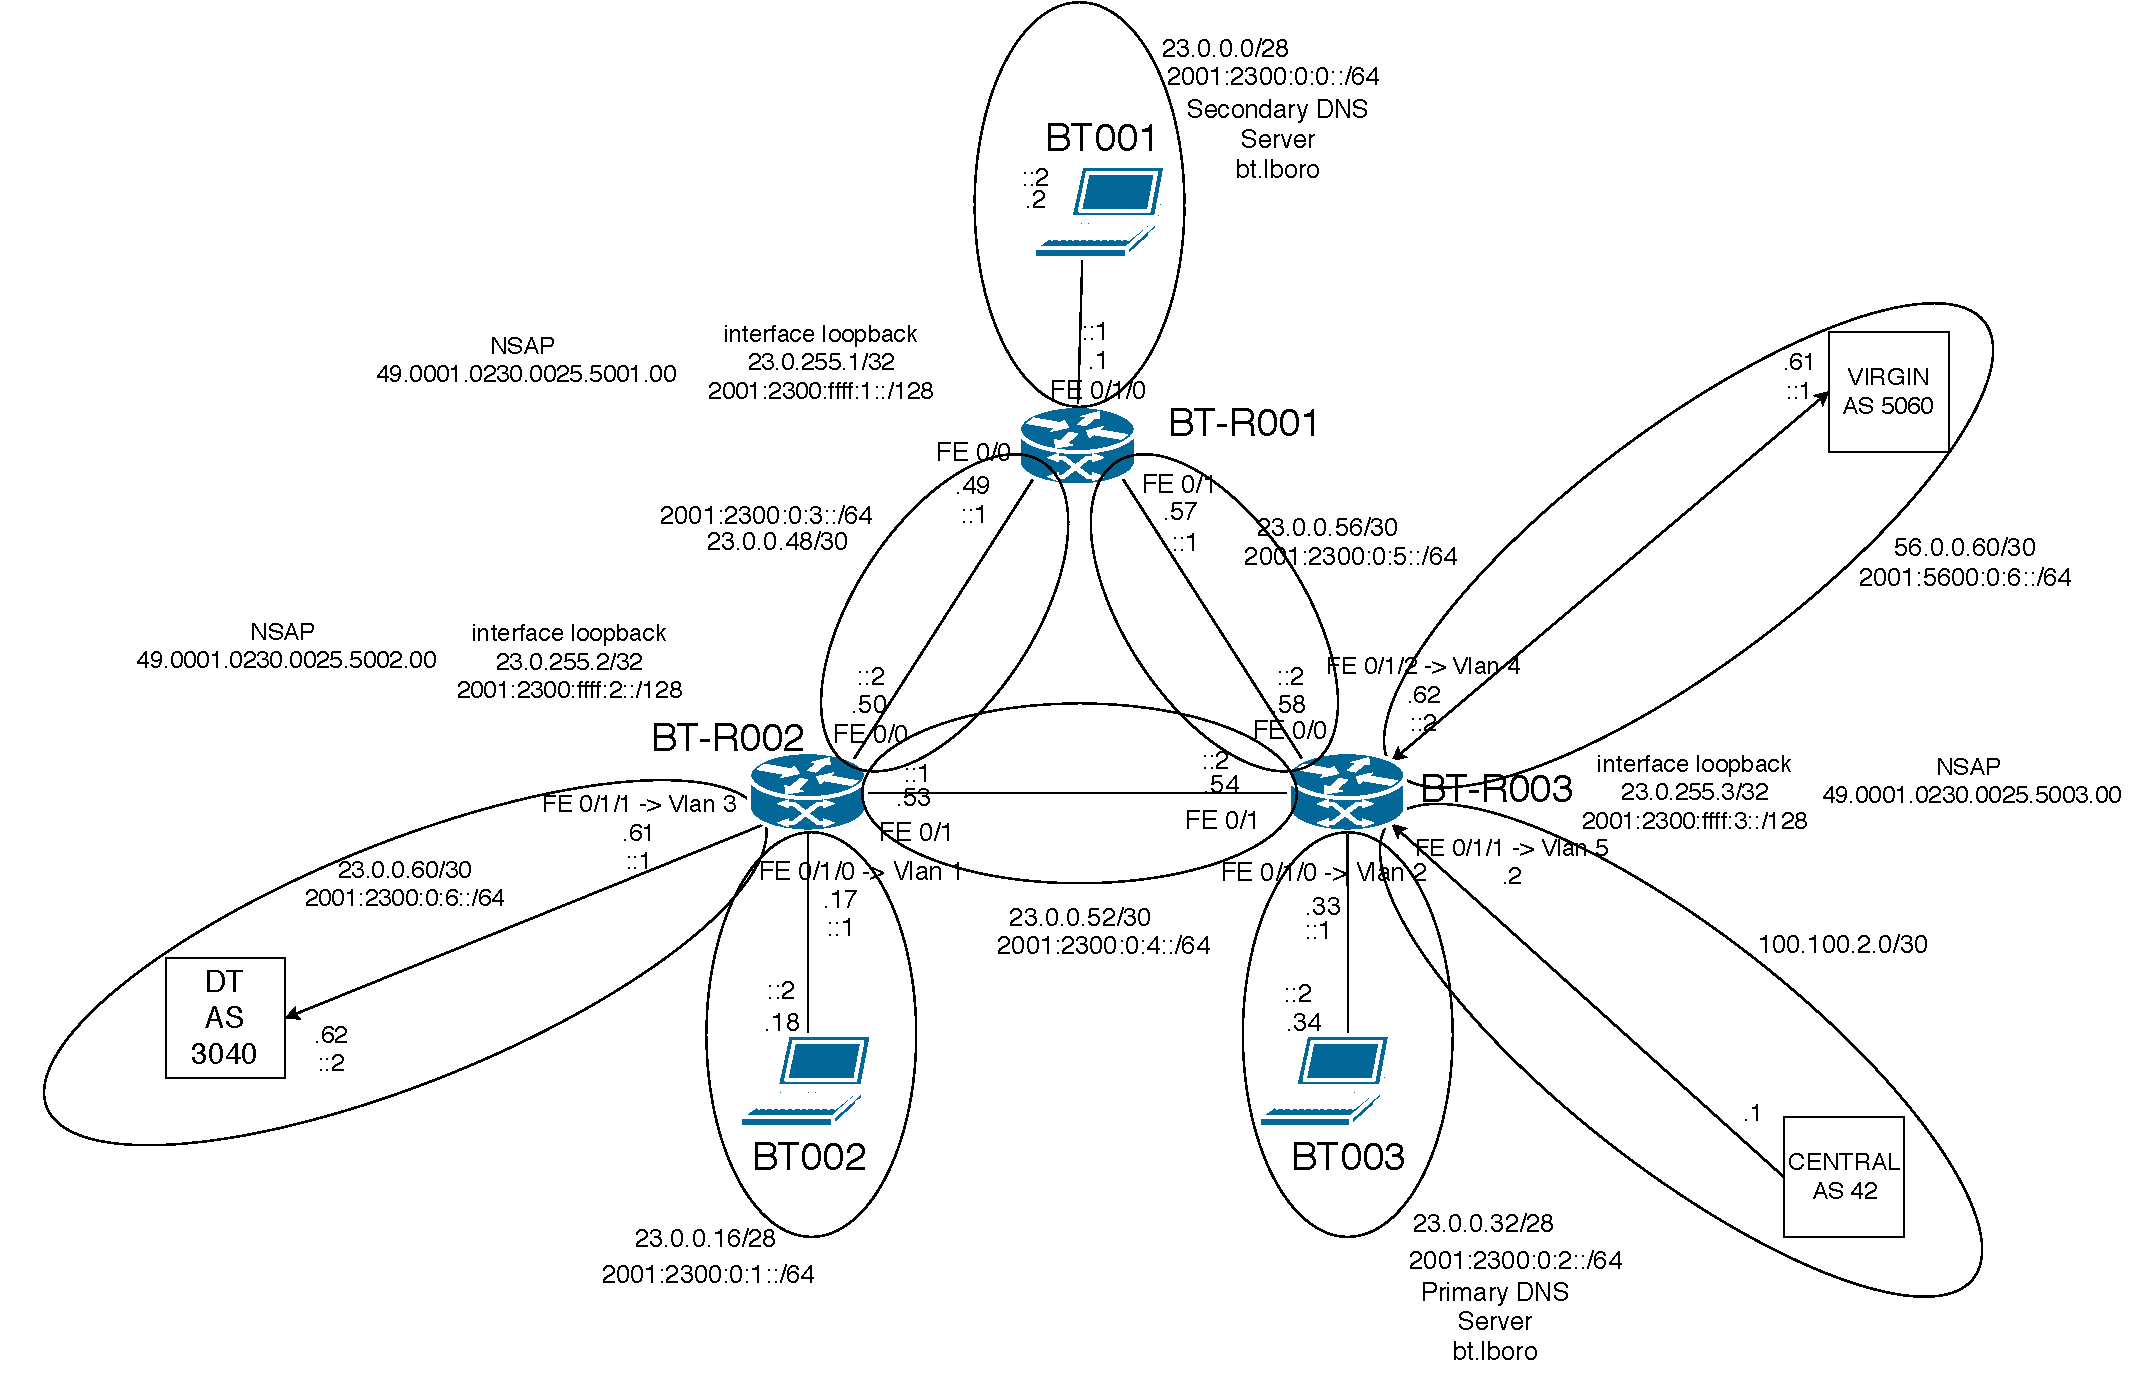
\includegraphics[width=\linewidth]{diagram}
    \caption{Full Network Diagram of BT Network.}
    \label{fig:diagram}
\end{figure}
\end{landscape}




\subsection{IP Addresses and Interfaces}

An IPv4 address range of \texttt{23.0.0.0/8} and IPv6 address range of \texttt{2001:2300::/32} are allocated to BT Network, which are further divided into sub-ranges to be allocated to each subnet.

For IPv4 addressing, a netmask of $n$ is needed for a subnet that demands $X$ host addresses, where $n$ is an integer that satisfies $2^{32-n} - 2 \geq X$ and $n \leq 32$. For our lab, the maximum value for netmask is used in order to minimize the size of each subnet and reserve address space for future customers. However, it's also possible to use a larger value for each Router-Laptop subnet in order to maximize the size of the subnet, given that the number of customers (in this case, $3$) is fixed.

In BT Network, the netmask for each Router-Router and Router-Neighbor subnet is $30$ while the netmask for each Router-Laptop subnet is $28$. In other words, each Router-Router and Router-Neighbor subnet has $2$ guaranteed IPv4 host addresses while each Router-Laptop subnet has $14$ guaranteed IPv4 host addresses. During address block allocation, larger subnet is being considered before smaller one reduce the number of block segments.

For IPv6 addressing, however, each subnet has a fixed netmask of $64$ to ensure that each interface in the subnet has a unique address. The full details of IP address allocation is shown in Table \ref{tab:ip}.

\begin{figure}[ht!]
    \centering
    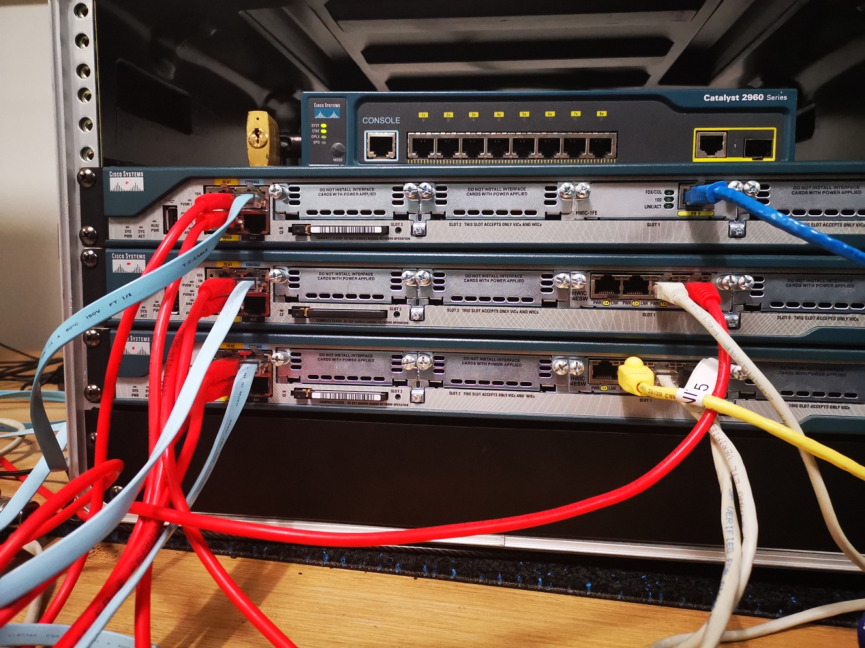
\includegraphics[width=0.8\linewidth]{physical}
    \caption{Physical Connections within BT Network.}
    \label{fig:physical}
\end{figure}

In terms of interfaces, there are $3$ Ethernet interfaces (\texttt{FastEthernet0/0}, \texttt{FastEthernet0/1} and \texttt{FastEthernet0/1/0}) on Router 1, each of which can be assigned with an IP address. On Router 2 and 3, however, there are $6$ Ethernet interfaces each and only $2$ of them (\texttt{FastEthernet0/0} and \texttt{FastEthernet0/1}) can be directly assigned with IP addresses. 
The remaining $4$ interfaces are link layer interfaces and thus does not possess any IP address.
To be assigned with an IP address, such an interface need to be assigned to an Virtual LAN (VLAN) to which the address is actually assigned.

Router-Router connections are established through either \texttt{FastEthernet0/0} or \texttt{FastEthernet0/1} interfaces on both ends while Router-Laptop and Router-Neighbor are through one of the remaining interfaces on the router end.
Since both interfaces are on the left-hand side of each router and such arrangement helps distinguishing between Router-Router connections and others easily as shown in Figure \ref{fig:physical}. Interfaces of both ends for each connection as well as their corresponding IP addresses are detailed in Table \ref{tab:interfaces}.

\begin{landscape}
\scriptsize{
\begin{longtable}[]{@{}lllll@{}}
\toprule
Subnet & IPv4 Address / Netmask & IPv4 Address Range & IPv6
Address / Netmask & IPv6 Address Range\tabularnewline
\midrule
\endhead
\texttt{BT-R001} - \texttt{BT001} & \texttt{23.0.0.0/28} &
\texttt{23.0.0.1} - \texttt{23.0.0.14} & \texttt{2001:2300:0:0::/64} &
\texttt{2001:2300:0:0::1} -
\texttt{2001:2300:0:0:ffff:ffff:ffff:fffe}\tabularnewline
\texttt{BT-R002} - \texttt{BT002} & \texttt{23.0.0.16/28} &
\texttt{23.0.0.17} - \texttt{23.0.0.30} & \texttt{2001:2300:0:1::/64} &
\texttt{2001:2300:0:1::1} -
\texttt{2001:2300:0:1:ffff:ffff:ffff:fffe}\tabularnewline
\texttt{BT-R003} - \texttt{BT003} & \texttt{23.0.0.32/28} &
\texttt{23.0.0.33} - \texttt{23.0.0.62} & \texttt{2001:2300:0:2::/64} &
\texttt{2001:2300:0:2::1} -
\texttt{2001:2300:0:2:ffff:ffff:ffff:fffe}\tabularnewline
\texttt{BT-R001} - \texttt{BT-R002} & \texttt{23.0.0.48/30} &
\texttt{23.0.0.49} - \texttt{23.0.0.50} & \texttt{2001:2300:0:3::/64} &
\texttt{2001:2300:0:3::1} -
\texttt{2001:2300:0:3:ffff:ffff:ffff:fffe}\tabularnewline
\texttt{BT-R002} - \texttt{BT-R003} & \texttt{23.0.0.52/30} &
\texttt{23.0.0.53} - \texttt{23.0.0.54} & \texttt{2001:2300:0:4::/64} &
\texttt{2001:2300:0:4::1} -
\texttt{2001:2300:0:4:ffff:ffff:ffff:fffe}\tabularnewline
\texttt{BT-R001} - \texttt{BT-R003} & \texttt{23.0.0.56/30} &
\texttt{23.0.0.57} - \texttt{23.0.0.58} & \texttt{2001:2300:0:5::/64} &
\texttt{2001:2300:0:5::1} -
\texttt{2001:2300:0:5:ffff:ffff:ffff:fffe}\tabularnewline
\texttt{BT-R002} - \texttt{DT} & \texttt{23.0.0.60/30} &
\texttt{23.0.0.61} - \texttt{23.0.0.62} & \texttt{2001:2300:0:6::/64} &
\texttt{2001:2300:0:6::1} -
\texttt{2001:2300:0:6:ffff:ffff:ffff:fffe}\tabularnewline
\texttt{BT-R003} - \texttt{Virgin} & \texttt{56.0.0.60/30} &
\texttt{56.0.0.61} - \texttt{56.0.0.62} & \texttt{2001:5600:0:6::/64} &
\texttt{2001:5600:0:6::1} -
\texttt{2001:5600:0:6:ffff:ffff:ffff:fffe}\tabularnewline
\texttt{BT-R003} - \texttt{Central} & \texttt{100.100.2.0/30} &
\texttt{100.100.2.1} - \texttt{100.100.2.2} & &\tabularnewline
\bottomrule
\caption{Allocation of IPv4 and IPv6 Addresses to Subnets in BT Network.}
\label{tab:ip}
\end{longtable}
}

\scriptsize{
\begin{longtable}[]{@{}lllllll@{}}
\toprule
Connection & Interface 1 & IPv4 Address & IPv6 Address & Interface 2 & IPv4 Address & IPv6
Address \tabularnewline
\midrule
\endhead
\texttt{BT-R001} - \texttt{BT001} & \texttt{BT-R001}:
\texttt{FastEthernet0/1/0} & \texttt{23.0.0.1} &
\texttt{2001:2300:0:0::1} & \texttt{BT001}: \texttt{eth0} &
\texttt{23.0.0.2} & \texttt{2001:2300:0:0::2}\tabularnewline
\texttt{BT-R002} - \texttt{BT002} & \texttt{BT-R002}:
\texttt{FastEthernet0/1/0} -\textgreater{} \texttt{Vlan\ 1} &
\texttt{23.0.0.17} & \texttt{2001:2300:0:1::1} & \texttt{BT002}:
\texttt{eth0} & \texttt{23.0.0.18} &
\texttt{2001:2300:0:1::2}\tabularnewline
\texttt{BT-R003} - \texttt{BT003} & \texttt{BT-R003}:
\texttt{FastEthernet0/1/0} -\textgreater{} \texttt{Vlan\ 2} &
\texttt{23.0.0.33} & \texttt{2001:2300:0:2::1} & \texttt{BT003}:
\texttt{eth0} & \texttt{23.0.0.34} &
\texttt{2001:2300:0:2::2}\tabularnewline
\texttt{BT-R001} - \texttt{BT-R002} & \texttt{BT-R001}:
\texttt{FastEthernet0/0} & \texttt{23.0.0.49} &
\texttt{2001:2300:0:3::1} & \texttt{BT-R002}: \texttt{FastEthernet0/0} &
\texttt{23.0.0.50} & \texttt{2001:2300:0:3::2}\tabularnewline
\texttt{BT-R002} - \texttt{BT-R003} & \texttt{BT-R002}:
\texttt{FastEthernet0/1} & \texttt{23.0.0.53} &
\texttt{2001:2300:0:4::1} & \texttt{BT-R003}: \texttt{FastEthernet0/1} &
\texttt{23.0.0.54} & \texttt{2001:2300:0:4::2}\tabularnewline
\texttt{BT-R001} - \texttt{BT-R003} & \texttt{BT-R001}:
\texttt{FastEthernet0/1} & \texttt{23.0.0.57} &
\texttt{2001:2300:0:5::1} & \texttt{BT-R003}: \texttt{FastEthernet0/0} &
\texttt{23.0.0.58} & \texttt{2001:2300:0:5::2}\tabularnewline
\texttt{BT-R002} - \texttt{DT} & \texttt{BT-R002}:
\texttt{FastEthernet0/1/1} -\textgreater{} \texttt{Vlan\ 3} &
\texttt{23.0.0.61} & \texttt{2001:2300:0:6::1} & \texttt{DT} &
\texttt{23.0.0.62} & \texttt{2001:2300:0:6::2}\tabularnewline
\texttt{BT-R003} - \texttt{Virgin} & \texttt{BT-R003}:
\texttt{FastEthernet0/1/2} -\textgreater{} \texttt{Vlan\ 4} &
\texttt{56.0.0.62} & \texttt{2001:5600:0:6::2} & \texttt{Virgin} &
\texttt{56.0.0.61} & \texttt{2001:5600:0:6::1}\tabularnewline
\texttt{BT-R003} - \texttt{Central} & \texttt{BT-R003}:
\texttt{FastEthernet0/1/1} -\textgreater{} \texttt{Vlan\ 5} &
\texttt{100.100.2.2} & & \texttt{Central} & \texttt{100.100.2.1}
&\tabularnewline
\bottomrule
\caption{Interfaces for Each Physical Connection and Corresponding IPv4 and IPv6 Addresses.}
\label{tab:interfaces}
\end{longtable}
}

\end{landscape}







% \chapter{Routing Protocols in the Network}
\label{chap:routing}




% \chapter{Applications in the Network}
\label{chap:applications}

\section{Secure Remote Access to Routers through SSH}

\subsection{Design}

Accessing the routers through the physical "console" port is inconvenient and dangerous. Thus, remote acess through Secure Shell (SSH) protocol to routers is needed. 

In our network, we enable remote SSH access on all 3 routers. We use seperate combinations of username and password on each router to ensure the independence of security of each router.

In addition, we set up SSH public key authentication on Laptop 1 (BT001), which allows the root user on the laptop to login in to all routers without entering passwords.

\subsection{Implementation}

We first set up remote SSH access as instructed in Reference Guide on all 3 routers. Below is the configuration commands for Router 1 (BT-R001).

\begin{lstlisting}
hostname BT-R001
ip domain name bt.lboro
username r001 priv 15 secret <secret>
line vty 0 4
transport input ssh telnet
login local

ip ssh version 2
crypto key generate rsa general-keys
ip ssh dh min size 4096
\end{lstlisting}

We then generate a pair of public and private keys on Laptop 1 (BT001).

\begin{lstlisting}
ssh-keygen
\end{lstlisting}

After that, the pair of keys is written into files
\texttt{\textasciitilde{}/.ssh/id\_rsa} and
\texttt{\textasciitilde{}/.ssh/id\_rsa.pub} . We use the generated
public key ( \texttt{id\_rsa.pub} ) to set up SSH public key
authentication on all 3 routers.

\begin{lstlisting}
ip ssh pubkey-chain
username r001
key-string
\end{lstlisting}

\subsection{Evaluation}

Once remote SSH access is set up on 3 routers, we should be able to access them on Laptop 1 (BT001) without entering the password using the following commands.

\begin{lstlisting}[language=sh]
# access Router 1
ssh r001@23.0.0.1 
# access Router 2
ssh r002@23.0.0.50
# access Router 3
ssh r003@23.0.0.33
\end{lstlisting}

Screenshots of successful remote access to all 3 routers are shown in Figure \ref{fig:ssh}.

\begin{figure*}[t!]
    \centering
    \begin{subfigure}[t]{0.3\textwidth}
        \centering
        \includegraphics[width=\linewidth]{ssh1}
        \caption{Router 1 (BT-R001)}
    \end{subfigure}
    ~ 
    \begin{subfigure}[t]{0.3\textwidth}
        \centering
        \includegraphics[width=\linewidth]{ssh2}
        \caption{Router 2 (BT-R002)}
    \end{subfigure}
    ~ 
    \begin{subfigure}[t]{0.3\textwidth}
        \centering
        \includegraphics[width=\linewidth]{ssh3}
        \caption{Router 3 (BT-R003)}
    \end{subfigure}
    \caption{Sucessful remote SSH access to all 3 routers from Laptop 1 (BT001).}
    \label{fig:ssh}
\end{figure*}


\subsection{Commentary}

\subsubsection{Problem: Maximum Limit of Characters per Line}

When we tried to set up SSH public key authentication on routers, we failed at our initial attempt. It turned out that Cisco router has maximum limit of characters for each command line. Thus, a public key in a single long line was not accepted by the router. 

To solve this problem, we then used \texttt{fold} command to split the public key into multiple lines before re-uploading the key and SSH public key authentication was successfully set up on the router.


\section{World Wide Web Service}

\subsection{Design}

\subsection{Implementation}

\subsection{Evaluation}

\subsection{Commentary}



\section{Domain Name System Service}

\subsection{Design}

\subsection{Implementation}

\subsection{Evaluation}

\subsection{Commentary}


\section{Email Service}

\subsection{Design}

\subsection{Implementation}

\subsection{Evaluation}

\subsection{Commentary}

% \chapter{Discussion}
\label{chap:discussion}

\section{Conclusions}
Several conclusions can be drawn from this lab.

\begin{enumerate}
\item
  BT Network, a small Tier-2 ISP, has been built and well tested. 
\item
  BT Network provides both intra-domain and inter-domain Internet connection to its users. It serves common Internet applications including Web, DNS and Email as well.
\item
  BT Network forms and implements business relationships with neighbouring ISPs.
\item
  Both IS-IS and BGP routing protocols can provide alternative route(s) to the destination when one of the physicial links is down.  
\end{enumerate}


\section{Further Work}

For the future, the following improvements are being considered.

\begin{enumerate}
\item
  Implement the alternative \textbf{next-hop solution} instead of "passive interface" as in Section \ref{sec:isis-alternative}.
\item
  Fully test the implementation of BGP routing in IPv6. We are unable to test it as no neighbouring ISP has set up IPv6 BGP routing as far as we know.
\item
  Provide other Internet services such as Dynamic Host Configuration Protocol (DHCP)\citep{rfc2131} and File Transfer Protocol (FTP)\citep{rfc959}.
\end{enumerate}



% \chapter{Contributions}
\label{chap:contributions}

\section{Group Leader: Zhihao DAI}

\section{Technical Director: Yunsong ZHANG}

\section{Network Engineer: Huijing LEI}

\section{Network Engineer: Changrong CHEN}

\section{Network Engineer: Yan HUANG}




\end{document}
